\begin{figure}[h!]
    \centering
    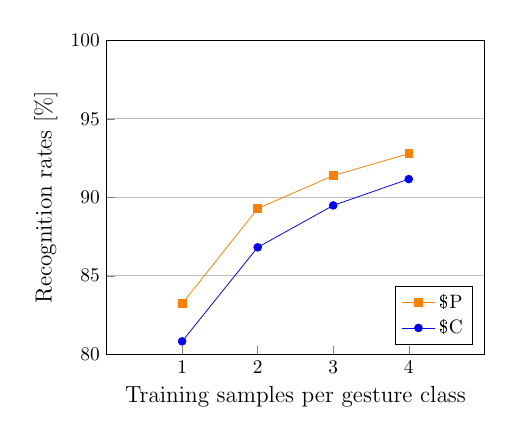
\begin{tikzpicture}[scale=.7]
        \begin{axis}[
            xlabel={\large{Training samples per gesture class}},
            ylabel={\large{Recognition rates [\%]}},
            xmin=0, xmax=5,
            ymin=80, ymax=100,
            xtick pos=bottom,
            ytick pos=left,
            xtick={1,2,3,4},
            ytick={80,85,90,95,100},
            legend pos=south east,
            ymajorgrids=true
        ]
            \addplot[color=orange,mark=square*]
                coordinates {(1, 83.22) (2, 89.28) (3, 91.38) (4, 92.78)};
            \addplot[color=blue,mark=*]
                coordinates {(1, 80.82) (2, 86.81) (3, 89.48) (4, 91.16)};
            \legend{\$P, \$C}
        \end{axis}
    \end{tikzpicture}%
    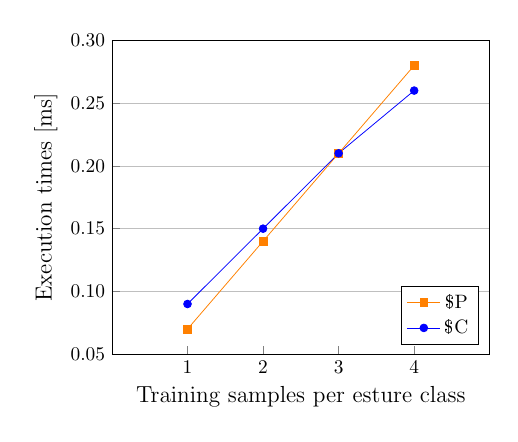
\begin{tikzpicture}[scale=.7]
        \begin{axis}[
            xlabel={\large{Training samples per esture class}},
            ylabel={\large{Execution times [ms]}},
            xmin=0, xmax=5,
            ymin=0.05, ymax=0.3,
            xtick pos=bottom,
            ytick pos=left,
            xtick={1,2,3,4},
            ytick={0.05,0.1,0.15,0.2,0.25,0.3},
            legend pos=south east,
            ymajorgrids=true,
            y tick label style={
                /pgf/number format/.cd,fixed,fixed zerofill,precision=2,/tikz/.cd
            }
        ]
            \addplot[color=orange,mark=square*]
                coordinates {(1, 0.07) (2, 0.14) (3, 0.21) (4, 0.28)};
            \addplot[color=blue,mark=*]
                coordinates {(1, 0.09) (2, 0.15) (3, 0.21) (4, 0.26)};
            \legend{\$P, \$C}
        \end{axis}
    \end{tikzpicture}
    \caption{User-dependent platform-independent testing of \$P and \$C in terms of recognition rates [\%] and execution times [ms] when the recognizers are trained with gestures performed on a smartphone and tested with gestures performed on a tablet.}
    \label{fig:cdollar_ud_pi_s}
\end{figure}